\documentclass[journal, a4paper]{IEEEtran}
\usepackage{graphicx,color,amssymb,amsmath,framed,clrscode,amsthm,  epstopdf, epsfig, enumerate, url}
\usepackage{balance}
\usepackage{cite}
%	\usepackage{algorithm}
%\usepackage{algpseudocode}
%\usepackage[dvisvgm, usenames, dvipsnames]{color}

\IEEEoverridecommandlockouts
% The preceding line is only needed to identify funding in the first footnote. If that is unneeded, please comment it out.
%\usepackage{cite}
\usepackage[font=scriptsize]{caption}
\usepackage[font=scriptsize]{subcaption}
%\usepackage{amsmath,amssymb,amsfonts}
\usepackage{csquotes}
\usepackage{paralist}
%\usepackage{multicol}
%\usepackage{lineno} 
\usepackage[switch]{lineno}
%\usepackage{flushend}



\usepackage{xcolor}


\pagestyle{empty}
%\usepackage{algorithm, algorithmic}
%\usepackage{algpseudocode}
\usepackage[ruled,vlined]{algorithm2e}
\usepackage{mathtools}
\DeclarePairedDelimiter\ceil{\lceil}{\rceil}
\DeclarePairedDelimiter\floor{\lfloor}{\rfloor}
%\setcounter{AlgoLine}{29}

\begin{document}
	
	\title{Analysis of Parallelized Memory Algorithms in High Performance Computing}
	

	%\author{Group 09: Prathyusha M R, Shreyas Udaya}

	\author{Group 09: Prathyusha M R , Shreyas Udaya	\\Department of Computer Science and Engineering \\ National Institute of Technology Karnataka\\ Surathkal, Mangalore-575025, Bharat \\ Email: prathyushamr.223cs500@nitk.edu.in, shreyasudaya.211cs152@nitk.edu.in}
	

	\maketitle
	
	% As a general rule, do not put math, special symbols or citations
	% in the abstract or keywords.
%	\begin{abstract}

		
		
%	\end{abstract}
	
	% Note that keywords are not normally used for peerreview papers.
%	\begin{IEEEkeywords}
	%	Flow accumulation; Parallel algorithms; OpenMP; Multicore processors
%	\end{IEEEkeywords}
	
	
	
	
	
	
	
	% page as needed:
	% \ifCLASSOPTIONpeerreview
	% \begin{center} \bfseries EDICS Category: 3-BBND \end{center}
	% \fi
	%
	% For peerreview papers, this IEEEtran command inserts a page break and
	% creates the second title. It will be ignored for other modes.
	\IEEEpeerreviewmaketitle
	
	
	
	
	\maketitle
	
	\thispagestyle{empty}
	\section{Introduction}

	Remote sensing technologies have increased geospatial data collection and resolution, which requires efficient computational algorithms to process big geographic information systems (GIS) data. This data is crucial for hydrological, topographic analysis, environmental modeling, and earth surface simulation. These models help understand complex environmental interactions, facilitating informed decision-making and policy formulation. Several algorithms are developed to support computational tasks in environmental modeling. However, with the increase in data size, calculating parameters on a single computer is not practical using serial algorithms \cite{CHO2023105771,KOTYRA2023105728}.
	
	Many researchers in geospatial data processing explored parallel algorithms to improve computational efficiency. Parallel programming utilizes modern parallel hardware in high-performance applications, including shared-memory architectures (like multicores) and distributed-memory architectures (like clusters). The complexity of this hardware is increasing due to out-of-order memory hierarchies, smart network interface cards and computing capabilities used as co-processors in various networking-related tasks \cite{LOFF2021743}.
	
	Parallel algorithms are used to improve computational efficiency by breaking down complex problems into manageable tasks that can be executed simultaneously using multiple processors. Techniques include OpenMP, MPI, GPGPU, and asynchronous many-tasks. OpenMP is an established framework for parallel programming \cite{KOTYRA2023105728}.
	
	OpenMP is the application programming interface (API) standard for parallel computing using shared memory. It provides directives for shared-memory parallelism, enabling developers to create efficient and scalable parallel algorithms. In OpenMP, the program is shared among several threads, where each thread executes a portion of the code concurrently. These threads work together effectively due to the coordinated access to shared memory. This framework is advantageous in providing the parallel capabilities of contemporary multicore processors. It improves the efficiency of algorithms and applications in various fields \cite{chapman2007using}.
	
	In environment modeling, the flow accumulation algorithm is a crucial tool in hydrology and GIS for understanding surface water movement. With flow accumulation calculations in a rasterized topographical model, the algorithm determines each cell's overall upstream contributing area in a digital elevation model. This method helps identify primary flow paths within a watershed and is essential for flood prediction, watershed management, and terrain analysis. Its sophisticated variations and adaptations continually refine our understanding of surface water behavior in diverse terrains \cite{CHO2023105771,KOTYRA2023105728,Zhou2019}.
	
	However, parallelization of flow accumulation tasks remains challenging due to spatial dependency and global computation. In this article, the weighted flow accumulation algorithm to calculate the longest flow path is parallelized using OpenMP and their performance is compared with the existing flow accumulation algorithm.
	
	%The flow accumulation algorithm presented in \cite{CHO2023105771} supports parallel computation using OpenMP. The source code can be found in \cite{r.flowaccumulation}.However, the algorithm used for calculating weighted flow accumulation and longest flow path \cite{CHO2020104774} does not support parallelization. The source code can be found in \cite{r.accumulate}. this work, we propose to parallelize the weighted flow accumulation algorithm 
	 
	

	
	The rest of this paper is organized as follows: Related works are reviewed in Section \ref{sec: ls}.  Section \ref{sec: pm} presents the methodology.
	
	
	
	
	\section{Related Works} 
	\label{sec: ls}
	
	This section provides an overview of the existing research \cite{ KOTYRA2021104741, DEJONG2022105083, CHO2020104774, stojanovic2020accelerating, 10.1007/978-3-030-60939-9_16,KOTYRA2023105613, HUANG2022106} in different parallel algorithms for flow accumulation calculation. It examines various approaches, evaluation methodologies, results, and the challenges they encountered in their respective studies.
	
	Kotyra \textit{et al.} \cite{KOTYRA2021104741} developed faster ways to calculate flow accumulation, resulting in shorter execution times. They suggested two approaches to parallelize flow accumulation algorithms: the bottom-up approach and the top-down approach. The study used 118 distinct data sets to compare six flow accumulation methods in sequential, parallel, and task-based implementations. The result inferred that the top-down algorithm was the fastest, with an average execution time of less than 30 seconds. For flow accumulation calculations, the parallel top-down implementation is observed to be the most suitable algorithm. The average processing time of task-based top-down implementation is 21.1\% longer for subcatchments and 32.7\% longer for rectangular frames, making it less efficient. The linear time complexity of the algorithm was measured in various settings, including frame 58 and frame 17, with 240 threads per core. Compared to the sequential version, the results showed a high correlation between the number of cores employed and the speedup. The increase in number of cores up to 60 led to reduced average computation time.

	Jong \textit{et al.} \cite{DEJONG2022105083} developed flow accumulation algorithms to determine how the material flows downstream. For parallel and concurrent computations, they employed the asynchronous many-task (AMT) approach. AMT helps to prevent synchronization points and increase the composability of modeling operations. The AMT-based algorithms were evaluated for composability, performance and scalability. It is observed that they function well when paired with other ooperationsand utilize additional hardware efficiently. However, further research is required ito optimizethe algorithms for particular hardware architectures and to assess their performance on larger datasets. The limitation is that the performance of the algorithms was assessed on a limited set of datasets. Also, further research is essential to examine the effects of different hardware architectures, flow direction algorithms, scheduling strategies and programming languages.
	
	Kotyra \textit{et al.} \cite{KOTYRA2023105728} designed seven fast raster-based algorithms to determine the longest flow paths in flow direction grids using a linear time complexity approach. Eight large datasets were used to evaluate the algorithm, which was generated using a hydrological model. The authors compared the algorithm using existing GIS software. Depending on the dataset and algorithm, the algorithms obtained significant speedups up to 30 times quicker on Windows and 17 times faster on Ubuntu. The suggested algorithm achieved fast and accurate results in determining the longest flow pathways in flow direction grids. However, their approach might not be applicable to unsteady flow conditions since it is based on raster data and a steady-state flow assumption. Future research should explore algorithms based on more complex models. Also, it should support the scalability and portability of their algorithms to other platforms and architectures.

	Cho \textit{et al.} \cite{CHO2020104774} proposed the longest flow path algorithm, which computes few rasters to enhance efficiency and decrease computation time. They developed an algorithm based on depth-first search and breadth-first search. The approach uses Hack's law-derived equations to estimate the longest flow length. In order to speed up traversal and eliminate inferior neighbor cells, the algorithm additionally uses a branching technique. The suggested method is evaluated through benchmark experiments conducted in Georgia and Texas, comparing the algorithm's performance with the Arc hydro longest flow path tool for ArcGIS Pro. The results showed that the algorithm's performance is affected by disk type and memory size, with solid-state drives and larger memory sizes resulting in faster computation times. The authors conclude that the proposed algorithm is valuable to environmental modeling and software. One limitation is that the experiments were conducted on a limited data set from two states in the United States. Furthermore, it is possible that the results may not be generalized to alternative geographical areas or datasets.  

	Stojanovic \textit{et al.} \cite{stojanovic2020accelerating} suggested accelerating the flow distribution phase using MPI on a cluster. The author suggested the parallelization of the flow distribution computation phase of the watershed analysis algorithm using MPI. Two different MPI implementations were discussed, along with the analysis of the advantages and challenges of both parallel implementations. The experimental evaluation is conducted on several large DEM datasets and varying numbers of computers in the cluster. They observed the approach that overlaps process computing and communication achieves the best results. The proposed MPI solutions effectively accelerate the flow accumulation step of watershed analysis. The speedup using MPI is significant compared to sequential execution. While these are effective, other methods are not considered, and neither are other libraries, such as OpenMP or CUDA.
	
	Lal \textit{et al.} \cite{10.1007/978-3-030-60939-9_16} presented a quantitative analysis on the caches for memory divergent workloads simulated by gpgpu-sim. Increasing the size of the L1 data cache improved the spatial locality while increasing L2 improved temporal locally. The authors analyzed the impact of parameters like block size and thread count on the algorithm's performance and optimized it on different hardware configurations. The evaluation is based on benchmarks run on an NVIDIA GPU. For memory-divergent tasks, the study focused on data locality in GPU caches. Higher inter-warp hits (46\%) at the L1 cache for memory-divergent workloads compared to the state-of-the-art. However, data over-fetch wastes around 50\% of cache capacity and other limited resources. The limitations include its focus on NVIDIA GPU architectures, its limited application to different types of workloads, and its inability to consider other potential performance bottlenecks.
	
	Kotyra \textit{et al.} \cite{KOTYRA2023105613} proposed a fast watershed delineation algorithm for GPU that uses OpenMP and CUDA. The algorithm iteratively processes each cell in the flow direction raster, identifying its downstream neighbor and checking if it belongs to the same catchment area. It includes optimizations to reduce memory usage and improve performance. The algorithm outperformed traditional GIS software packages in terms of speed and efficiency. The algorithm's main loop calls the GPU kernel repeatedly, accounting for an average of 28.8\% of the overall execution time. Data transfers account for 34.5\% of the total time on average. The choice of hardware and software platforms affects the algorithm's performance, and its implementation may require specialized knowledge in parallel programming and GPU computing.
	
	Huang \textit{et al.} \cite{HUANG2022106} discussed a comprehensive study of in-memory computing.	They discussed portability, robustness, usability, and performance of software. The evolution of in-memory computing is explained. The authors suggested they commit history for two in-memory libraries and observed most of the commits	were towards performance maintenance, suggesting it has a significant role in computation. The in-memory computing has better performance than traditional post-processing. The portability, robustness, usability, and implementation of software are all considered in the evaluation of performing in-memory computing. The results suggest that in-memory computing provides significantly better performance and scalability than traditional post-processing.
	
	\begin{table*}[]
		\centering
		\begin{tabular}{ | p{0.7cm} | p{1cm} | p{2.5cm} | p{2.5cm} | p{2.5cm} |  p{2.5cm} |p{2.5cm} | }
			
			\hline
			\textbf{SI No.} &  \textbf{Authors} & \textbf{Approach} & \textbf{Evaluation} & \textbf{Results} & \textbf{Observation} & \textbf{Limitations}\\
			\hline
			1     &  Kotyra \textit{et al.} \cite{KOTYRA2021104741}& Two main approaches are discussed in o parallelize flow accumulation algorithms: the bottom-up approach and the top-down approach.  &  Using 118 distinct data sets, the study compared six flow accumulation methods in sequential, parallel, and task-based implementations. &	 The result inferred that the top-down algorithm was fastest, with an average execution time of less than 30 seconds. & Compared to sequential version, the results showed a high correlation between the number of cores employed and the speedup. & The study focused primarily on the development and evaluation of flow accumulation algorithms. \\
			\hline
			2     &  Jong \textit{et al.} \cite{DEJONG2022105083} & The authors  developed flow accumulation algorithms to determine how the material flows downstream.&  The AMT-based algorithms were evaluated for composability, performance and scalability. & The AMT-based algorithms for flow accumulation operations perform well in terms of scalability and composability .  & The algorithm function well when paired with other operations and utilize additional hardware efficiently. & The limitation is that the performance of the algorithms was assessed on a limited set of datasets.\\
			\hline
			3     &  Kotyra \textit{et al.} \cite{KOTYRA2023105728} & Seven fast raster-based algorithms to determine the longest flow paths in flow direction grids using a linear time complexity approach. & Eight large datasets were used to evaluate the algorithm which was generated using a hydrological model.& The algorithms obtained significant speedups of up to 30 times quicker on Windows and 17 times faster on Ubuntu. & The suggested algorithm performed well in achieving fast and accurate result in determining longest flow pathways in flow direction grids.& However, this approach might not be applicable unsteady flow conditions since it is based on raster data and a steady-state flow assumption.\\
			\hline
			4      & Cho \textit{et al.} \cite{CHO2020104774} & The longest flow path algorithm that computes a small number of rasters to enhance efficiency and decrease computation time  & The suggested method is evaluated through benchmark experiments conducted in Georgia and Texas, comparing the performance of the algorithm with the Arc hydro longest flow path tool for ArcGIS Pro.& The algorithm's performance is affected by disk type and memory size, with solid-state drives and larger memory sizes resulting in faster computation times.  & In order to speedup traversal and eliminate inferior neighbor cells, the algorithm additionally uses branching technique. &  One limitation is that the experiments were conducted on a limited set of data from two states in the United States.\\
			\hline
		
			5     &  Huang \textit{et al.} \cite{HUANG2022106} & The author presented comprehensive study of in-memory computing.They discussed portability, robustness, usability, and performance of software &  The authors quantitatively examined the workflow end-to-end time and evaluate with realistic workflows & The results suggested that in-memory computing offers much higher scalability and performance than the traditional post-processing. & Most of the commits were towards performance maintenance, suggesting it has a significant role towards computation. & One limitation is the availability of RDMA resources, which can constrain the maximum concurrency of RDMA memory requests.\\
			\hline
			6     &  Kotyra \textit{et al.} \cite{KOTYRA2023105613}& The author proposed a fast watershed delineation algorithm for GPU. that uses OpenMP and CUDA. &  The author evaluated the proposed algorithm using several experiments on different datasets and hardware configurations. &The results showed that the algorithm outperformed traditional GIS software packages in terms of speed and efficiency.  & The algorithm's performance is affected by the choice of hardware and software platforms. & One limitation is that the algorithm may not be suitable for all types of GIS-related problems. \\
			\hline
			7     & 	Stojanovic \textit{et al.} \cite{stojanovic2020accelerating} & The author suggested accelerating the flow distribution phase using MPI on a cluster. &  The experimental evaluation is conducted on several large DEM datasets and varying numbers of computers in the cluster. & The approach overlaps process computing and communication achieves the best results. & Two different MPI implementations were discussed along with the analysis on advantages and challenges of both parallel implementations. &  One limitation is that the study does not cover other parallel and distributed computing methods and technologies that can be used for geospatial data processing and analysis\\
			\hline
			8     &  Lal \textit{et al.} \cite{10.1007/978-3-030-60939-9_16}& The author  presented a quantitative analysis on the caches for memory divergent workloads simulated by gpgpu-sim. & The evaluation is based on benchmarks run on an NVIDIA GPU. The mpact of parameters like block size and thread count on the algorithm's performance  were analysed. & Higher inter-warp hits (46\%) at the L1 cache for memory-divergent workloads compared to the state-of-the-art. & Data over-fetch wastes around 50\% of cache capacity and other limited resources. & The limitations include its focus on NVIDIA GPU architectures, its limited application to other types of workloads, and its inability to consider other potential performance bottlenecks.\\
		\hline
	\end{tabular}
\end{table*}
	
	\section{Proposed Methodology}
	\label{sec: pm}
%	We want to create a new memory flow accumulation algorithm with 
%Section III must detail your approach, flowchart, algorithm, necessary mathematical expression, diagrams, tables, etc. 
	
	The flow accumulation algorithm is a crucial tool in hydrology and GIS for understanding surface water movement. This method helps to identify primary flow paths within a watershed and is essential for flood prediction,	watershed management, and terrain analysis. 
	
	The flow accumulation algorithms suggested in \cite{KOTYRA2021104741, DEJONG2022105083, KOTYRA2023105728, HUANG2022106, KOTYRA2023105613, stojanovic2020accelerating} has been a significant advancement in the domain of environmental modeling. These algorithms are parallelized using OpenMP to support computational tasks in environmental modeling. The parallelization of these algorithms enables the distribution of computational tasks across multiple processors or cores, resulting in accelerated processing times and improved performance.
	
	However, the weighted flow accumulation algorithm proposed in \cite{CHO2020104774} does not support parallelization. The goal of parallelizing the weighted flow accumulation technique is to enable concurrent computation, utilizing the power of multi-core processors and speeding up the computation of the longest flow path. This adaption is essential to ensure that the algorithms can effectively handle the complexities inherent in large-scale geospatial analyses and to satisfy the growing demands for faster and more scalable environmental modeling processes. This work focuses on parallelizing the weighted flow accumulation technique using OpenMP to determine the longest flow path.
	
	\subsection{GRASS GIS modules}
	
	Spatial data and information are integrated by Geographic Information Systems (GIS) software. It provides a structural framework for comprehending and analyzing geographical patterns. Environmental modeling is facilitated by GIS through the integration of multiple layers of data, including demographic data, satellite imagery, and maps. The Geographical Resources Analysis Support System (GRASS) is an open source GIS utilized for the generation, analysis, and mapping of geospatial data \cite{NETELER2012124}. GRASS GIS is utilized to process the GIS data in this study. It features a comprehensive collection of tools for vector, raster, and geospatial modeling.
	
	\subsection{Flow Accumulation Algorithm Comparison }
	
	GRASS GIS modules facilitate the modeling of raster-based environments. The flow accumulation is computed by the r.flowaccumulation module in GRASS through the utilization of the Memory-Efficient Flow Accumulation (MEFA) parallel algorithm on a flow direction raster map \cite{CHO2023105771, r.flowaccumulation}. This algorithm tracks and accumulates the quantity of flow draining through and including each cell by utilizing a flow direction raster map.

	The r.accumulate algorithm is recommended for the purpose of weighted flow accumulation. Using a flow direction map, the r.accumulate module computes weighted flow accumulation, subwatersheds, stream networks, and longest flow trajectories. In order to determine and compile the volume of flow passing through and encompassing each cell, this module exclusively employs a flow direction map \cite{CHO2020104774, r.accumulate}.
	
	The r.flowaccumulation algorithm  supports parallel computation of flow accumulation using OpenMP while the r.accumulate algorithm does not. 
	

	\subsection{Considerations for parallelizing weighted flow accumulation}
	 
	In order to optimize the implementation of the weighted flow accumulation algorithm when it is parallelized, careful consideration is required. To begin with, it is imperative to conduct a comprehensive examination of the algorithm's intricacy and intrinsic dependencies in order to detect possible opportunities for parallelization. In order to prevent resource under utilization and ensure an equitable distribution of computational tasks across processors or cores, effective load balancing becomes crucial. Furthermore, a meticulous examination of memory access patterns aids in the reduction of data movement and the enhancement of cache coherence. When evaluating shared-memory systems, the selection of a suitable parallelization framework, such as OpenMP, is crucial, taking into account the properties of the algorithm and the underlying hardware architecture. Ensuring minimal communication latency between parallel threads is crucial in order to prevent the advantages of parallelization from being offset. Scalability is a critical factor in determining the efficacy of an algorithm when confronted with problems of different sizes and computational capacities. The accuracy of the parallelized algorithm is ensured by exhaustive validation against the sequential version and robust error management and debugging mechanisms.  
	 
	\subsection{Problem specification}
	
	When attempting to determine the longest flow path, the substantial amount of time required to process raster data input presents an inherent difficulty, frequently impeding environmental modeling. Although completely avoiding the use of raster data is impractical, this study presents an alternative approach to this problem. Rewriting the recursive definition of the longest flow path so that it is expressed in terms of the upstream neighbor cells of the flow direction raster map. Notwithstanding its apparent simplicity, the recursive definition poses computational difficulties on account of the exponential growth in potential upstream cells, which is dependent on variables such as the size of the watershed and its topography. An equation is used to estimate the number of cells to visit at each stage, and constraints are investigated in order to efficiently eliminate non-candidate neighbor cells. Notwithstanding these endeavors, the authors concede that the computational efficiency is inadequate in comparison to a method based on flowlength. This emphasizes the intricacies involved in handling the exponential expansion of cells while performing the recursive computation of the longest flow path. 
	
	For implementing recursive longest flow path tracing, the pseudocode of the  procedure is shown in algorithm \ref{algo:1} and its subroutine is shown in algorithm \ref{algo:2}, respectively. The pseudocode for the iterative procedure and its subroutine that iteratively implements longest flow path tracing with a stack as its primary data structure for neighbor cell management is provided in algorithms \ref{algo:3} and \ref{algo:4}. Iterative  and recursive longest flow path algorithms are implemented by the r.accumulate GRASS GIS module. The programming language utilized for this module is C. In order to distinguish the two algorithms contained within the GRASS GIS module, the recursive and iterative implementations shall be denoted, respectively, as r. accumulate-recursive and r. accumulate-iterative. These two algorithms are both parallelized through the use of OpenMP directives.
	
	
	
	\begin{figure}[]
		\centering
		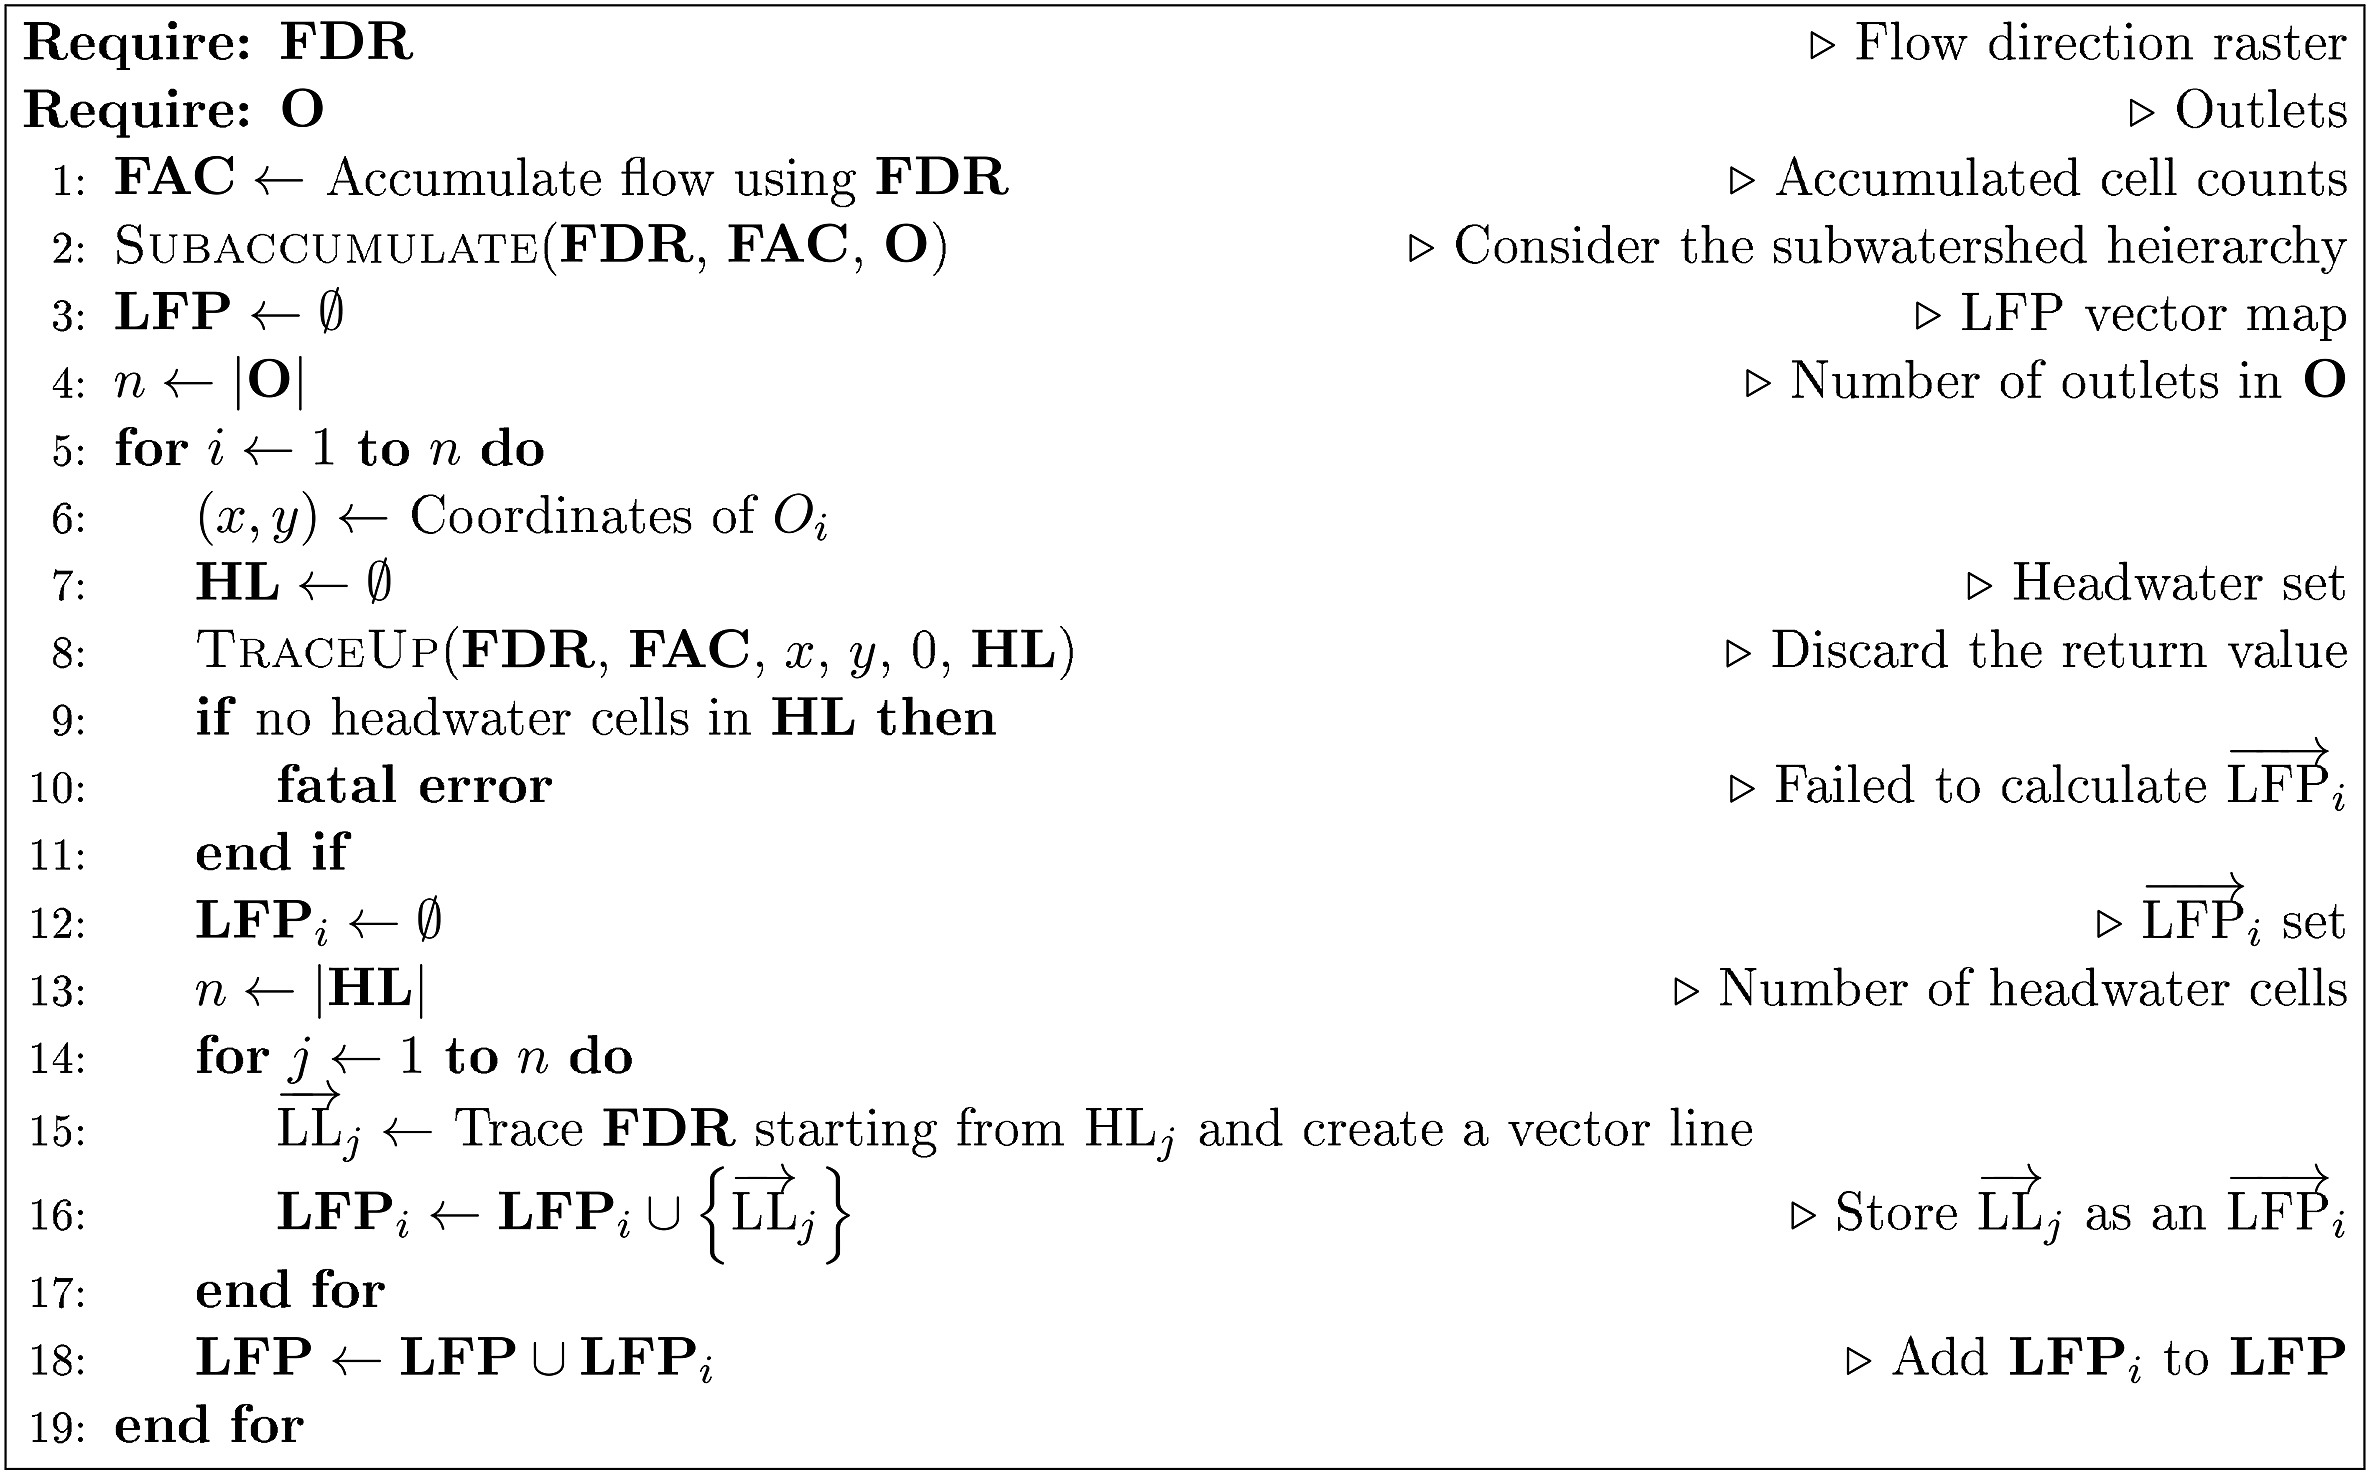
\includegraphics[width=0.5\textwidth]{./fig/Algorithm 4.jpg} \hspace*{\fill}
		\captionof{algocf}{ Pseudocode for r.accumulate-recursive }
		\label{algo:1}
	\end{figure}
	
	\begin{figure}[]
		\centering
		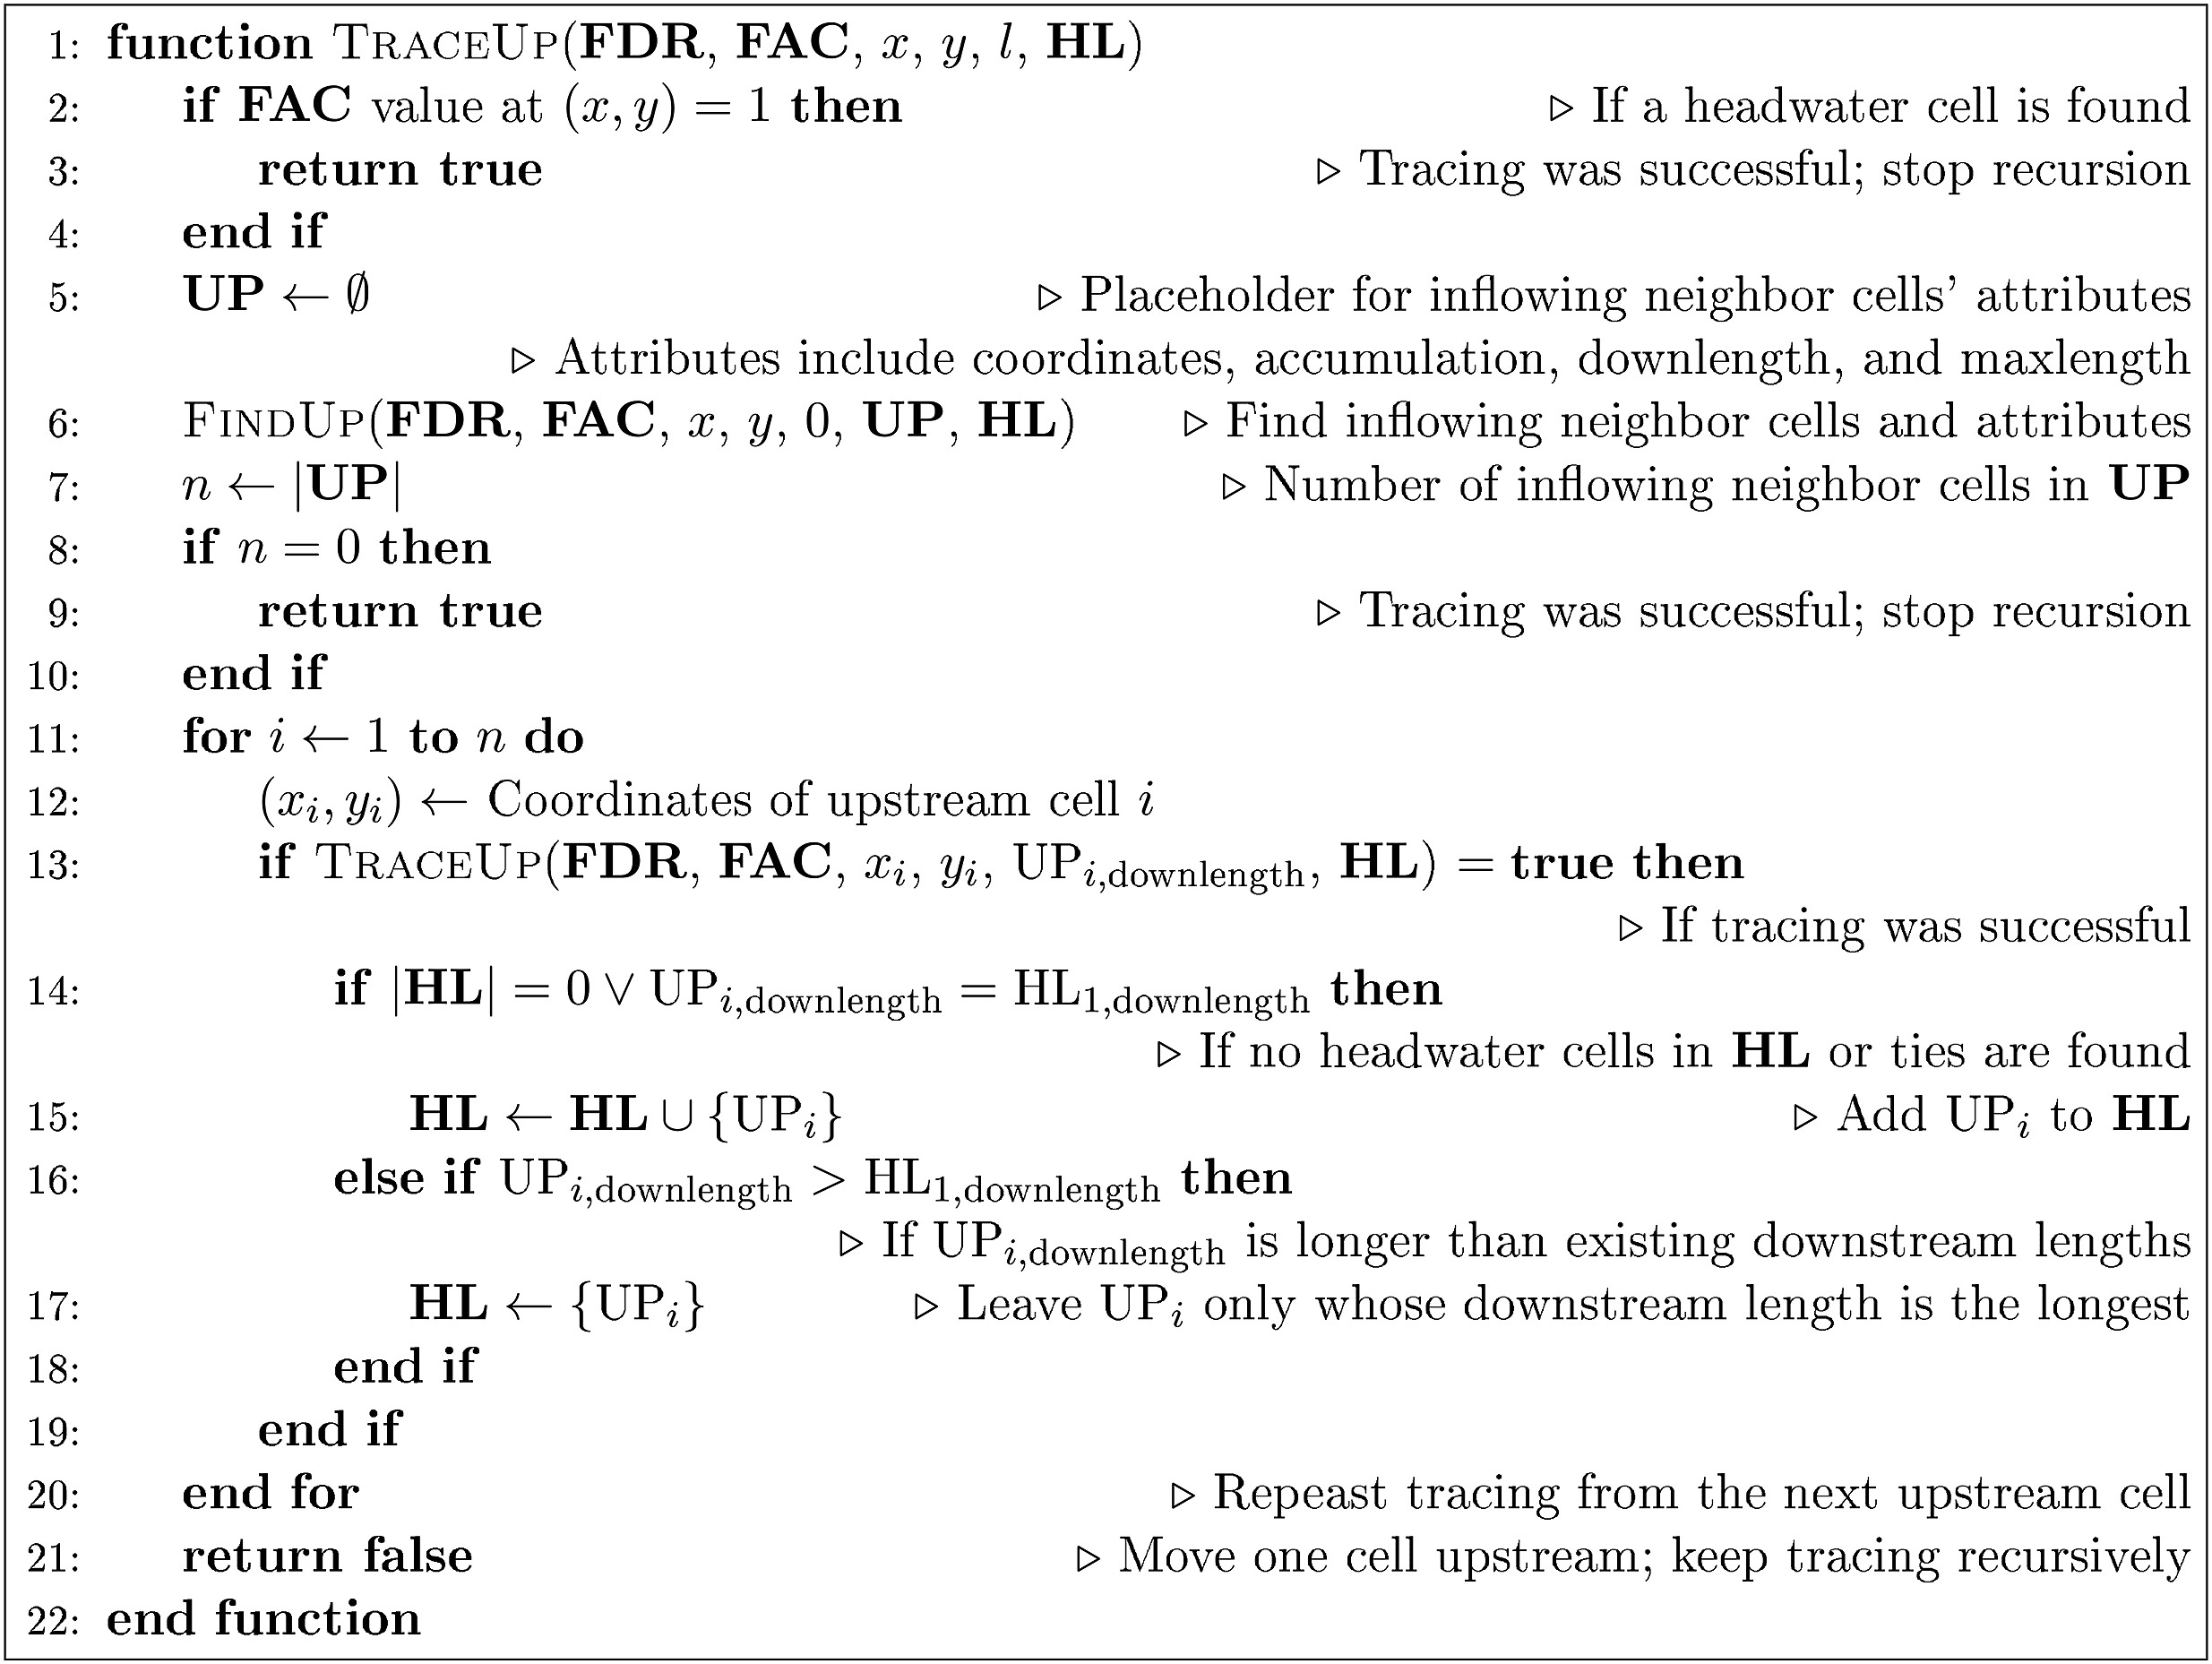
\includegraphics[width=0.5\textwidth]{./fig/Algorithm 5.jpg} \hspace*{\fill}
		\captionof{algocf}{ Pseudocode for the TraceUp function for r.accumulate-recursive. }
		\label{algo:2}
	\end{figure}

	\begin{figure}[]
		\centering
		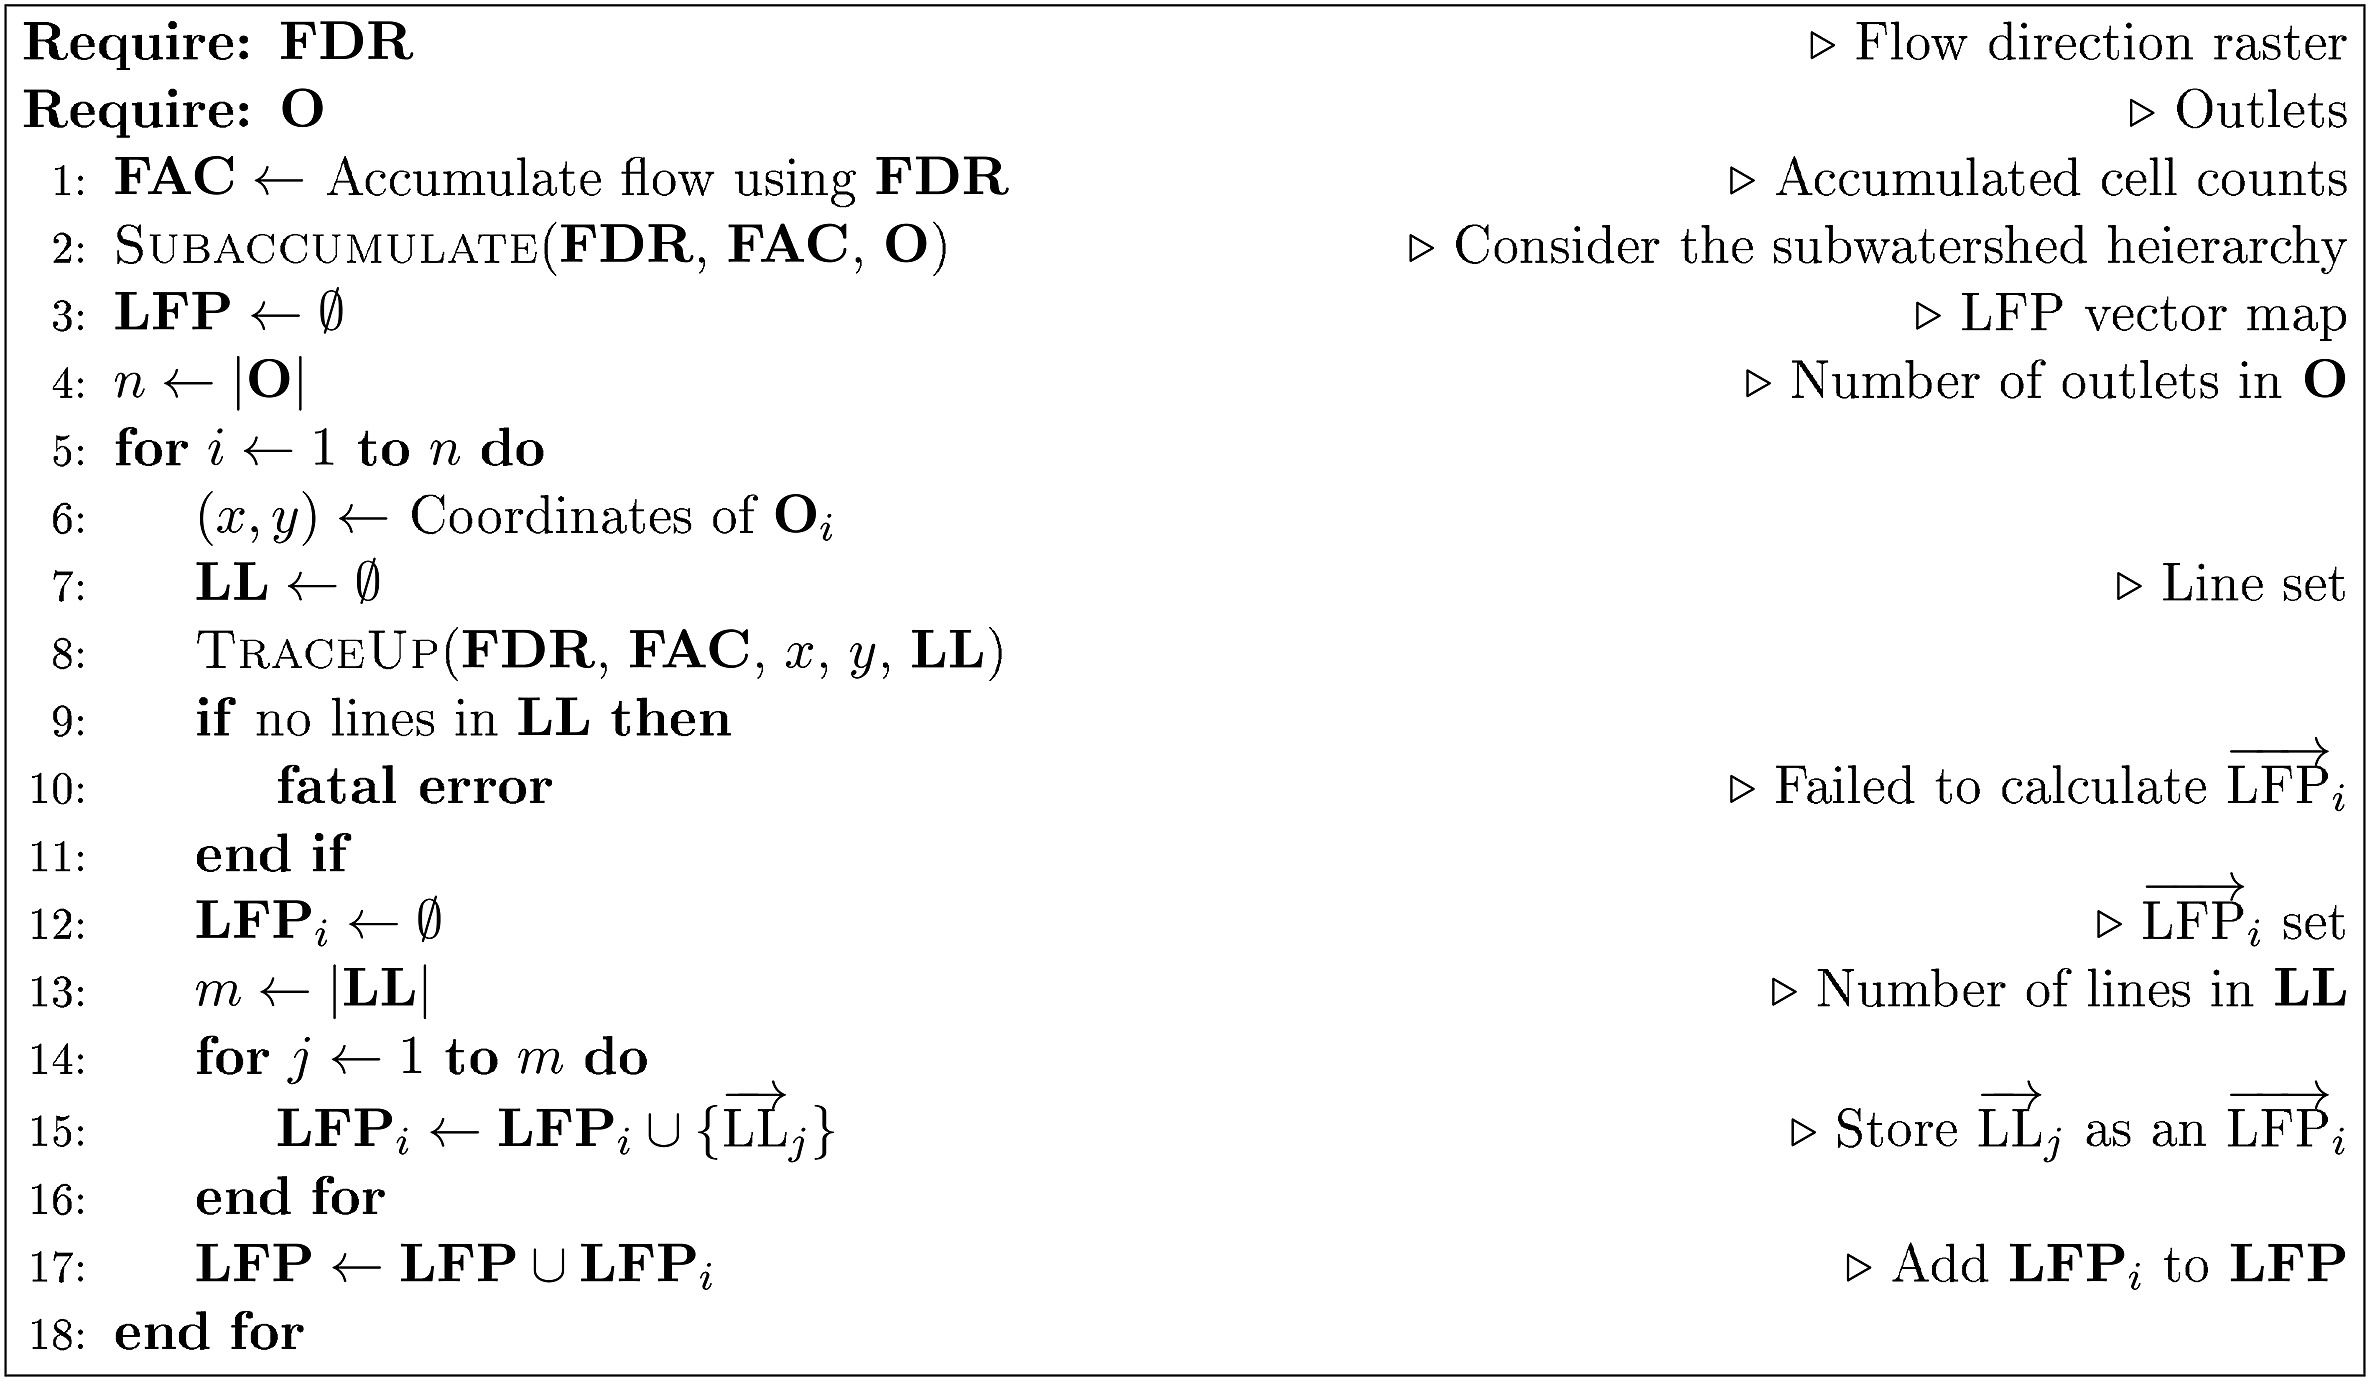
\includegraphics[width=0.5\textwidth]{./fig/Algorithm 6.jpg} \hspace*{\fill}
		\captionof{algocf}{ Pseudocode for r.accumulate-iterative.}
		\label{algo:3}
	\end{figure}

	\begin{figure}[]
		\centering
		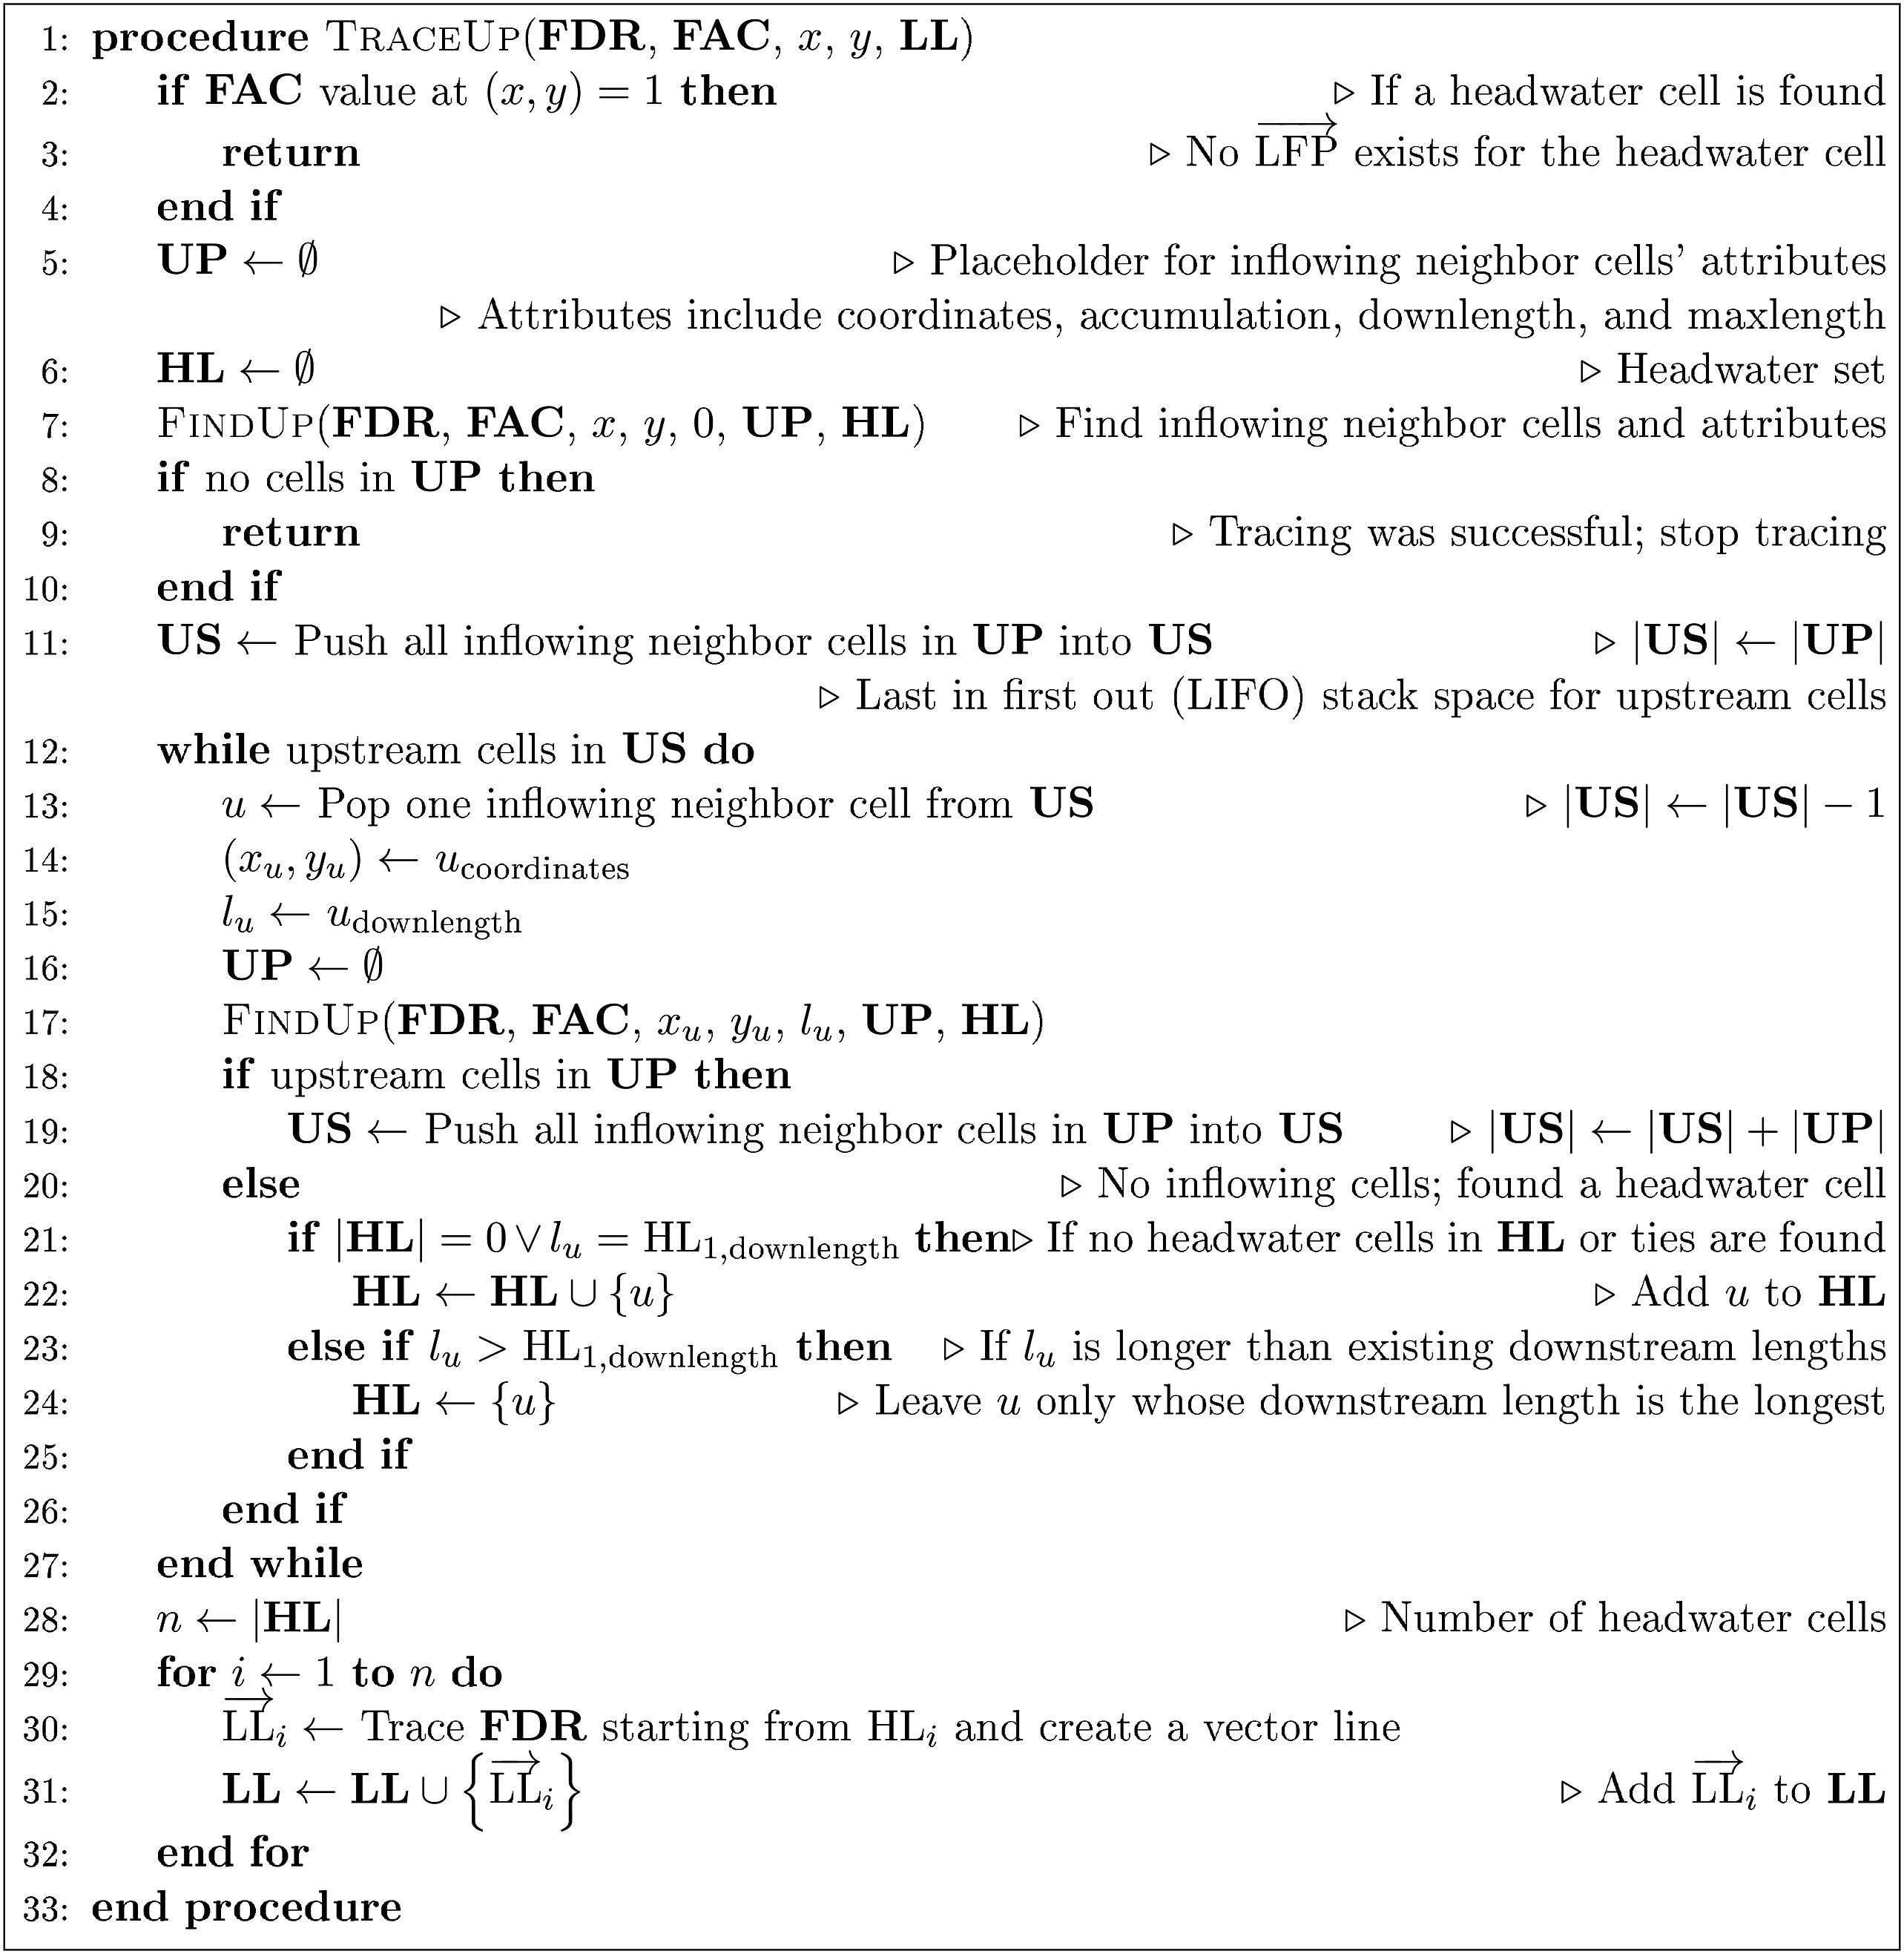
\includegraphics[width=0.5\textwidth]{./fig/Algorithm 7.jpg} \hspace*{\fill}
		\captionof{algocf}{ Pseudocode for the TraceUp function for r.accumulate-iterative. }
		\label{algo:4}
	\end{figure}
	
	\bibliographystyle{ieeetr}
	\bibliography{reference}

\end{document}